\documentclass{article} 
\usepackage[utf8]{inputenc} 
\usepackage[russian]{babel} 
\usepackage{graphicx} 
\usepackage{csvsimple} 
\usepackage{geometry} 
\usepackage{amsmath, amsfonts} 
\usepackage{setspace} 
\usepackage{pdfpages} 
\usepackage{listings} 

\graphicspath{{pictures/}}
\DeclareGraphicsExtensions{.pdf,.png,.jpg}

\lstset{breaklines=true} 
\pagestyle{empty}

\geometry{ 
  a4paper, 
  total={170mm,237mm}, 
  left=20mm, 
  top=20mm, 
} 

\begin{document}
\begin{titlepage}
    \begin{center}
    \textsc{МИНИСТЕРСТВО ОБРАЗОВАНИЯ И НАУКИ РОССИЙСКОЙ ФЕДЕРАЦИИ ФЕДЕРАЛЬНОЕ ГОСУДАРСТВЕННОЕ АВТОНОМНОЕ ОБРАЗОВАТЕЛЬНОЕ УЧРЕЖДЕНИЕ ВЫСШЕГО ОБРАЗОВАНИЯ\\[5mm]
    «Санкт–Петербургский национальный исследовательский университет информационных технологий, механики и оптики»\\[20mm]
    Факультет информационных технологий и программирования\\[5mm]
    }
    \vfill
    
    \textbf{ОБЪЕКТНО-ОРИЕНТИРОВАННОЕ ПРОГРАММИРОВАНИЕ\\[2mm]}
    \textbf{Мобильное приложение\\[20mm]}
    \end{center}
    
    \hfill
    \begin{minipage}{.3\textwidth}
    Выполнил студент:\\[2mm] 
    Ершов Михаил Николаевич \\
    группа: M3206\\[5mm]
    \end{minipage}%
    \vfill
    \begin{center}
    Санкт-Петербург, 2019 г.
    \end{center}
    \end{titlepage}

    \section{Постановка задачи}
    Приложение для android, которое позволяет отобразить карту, отметить точку на карте или точки, каждая точка имеет имя.
    Если телефон находится в радиусе, который задает юзер, то формируется электронное письмо с координатами телефона и точки.
    \section{Итог. Скриншоты}
    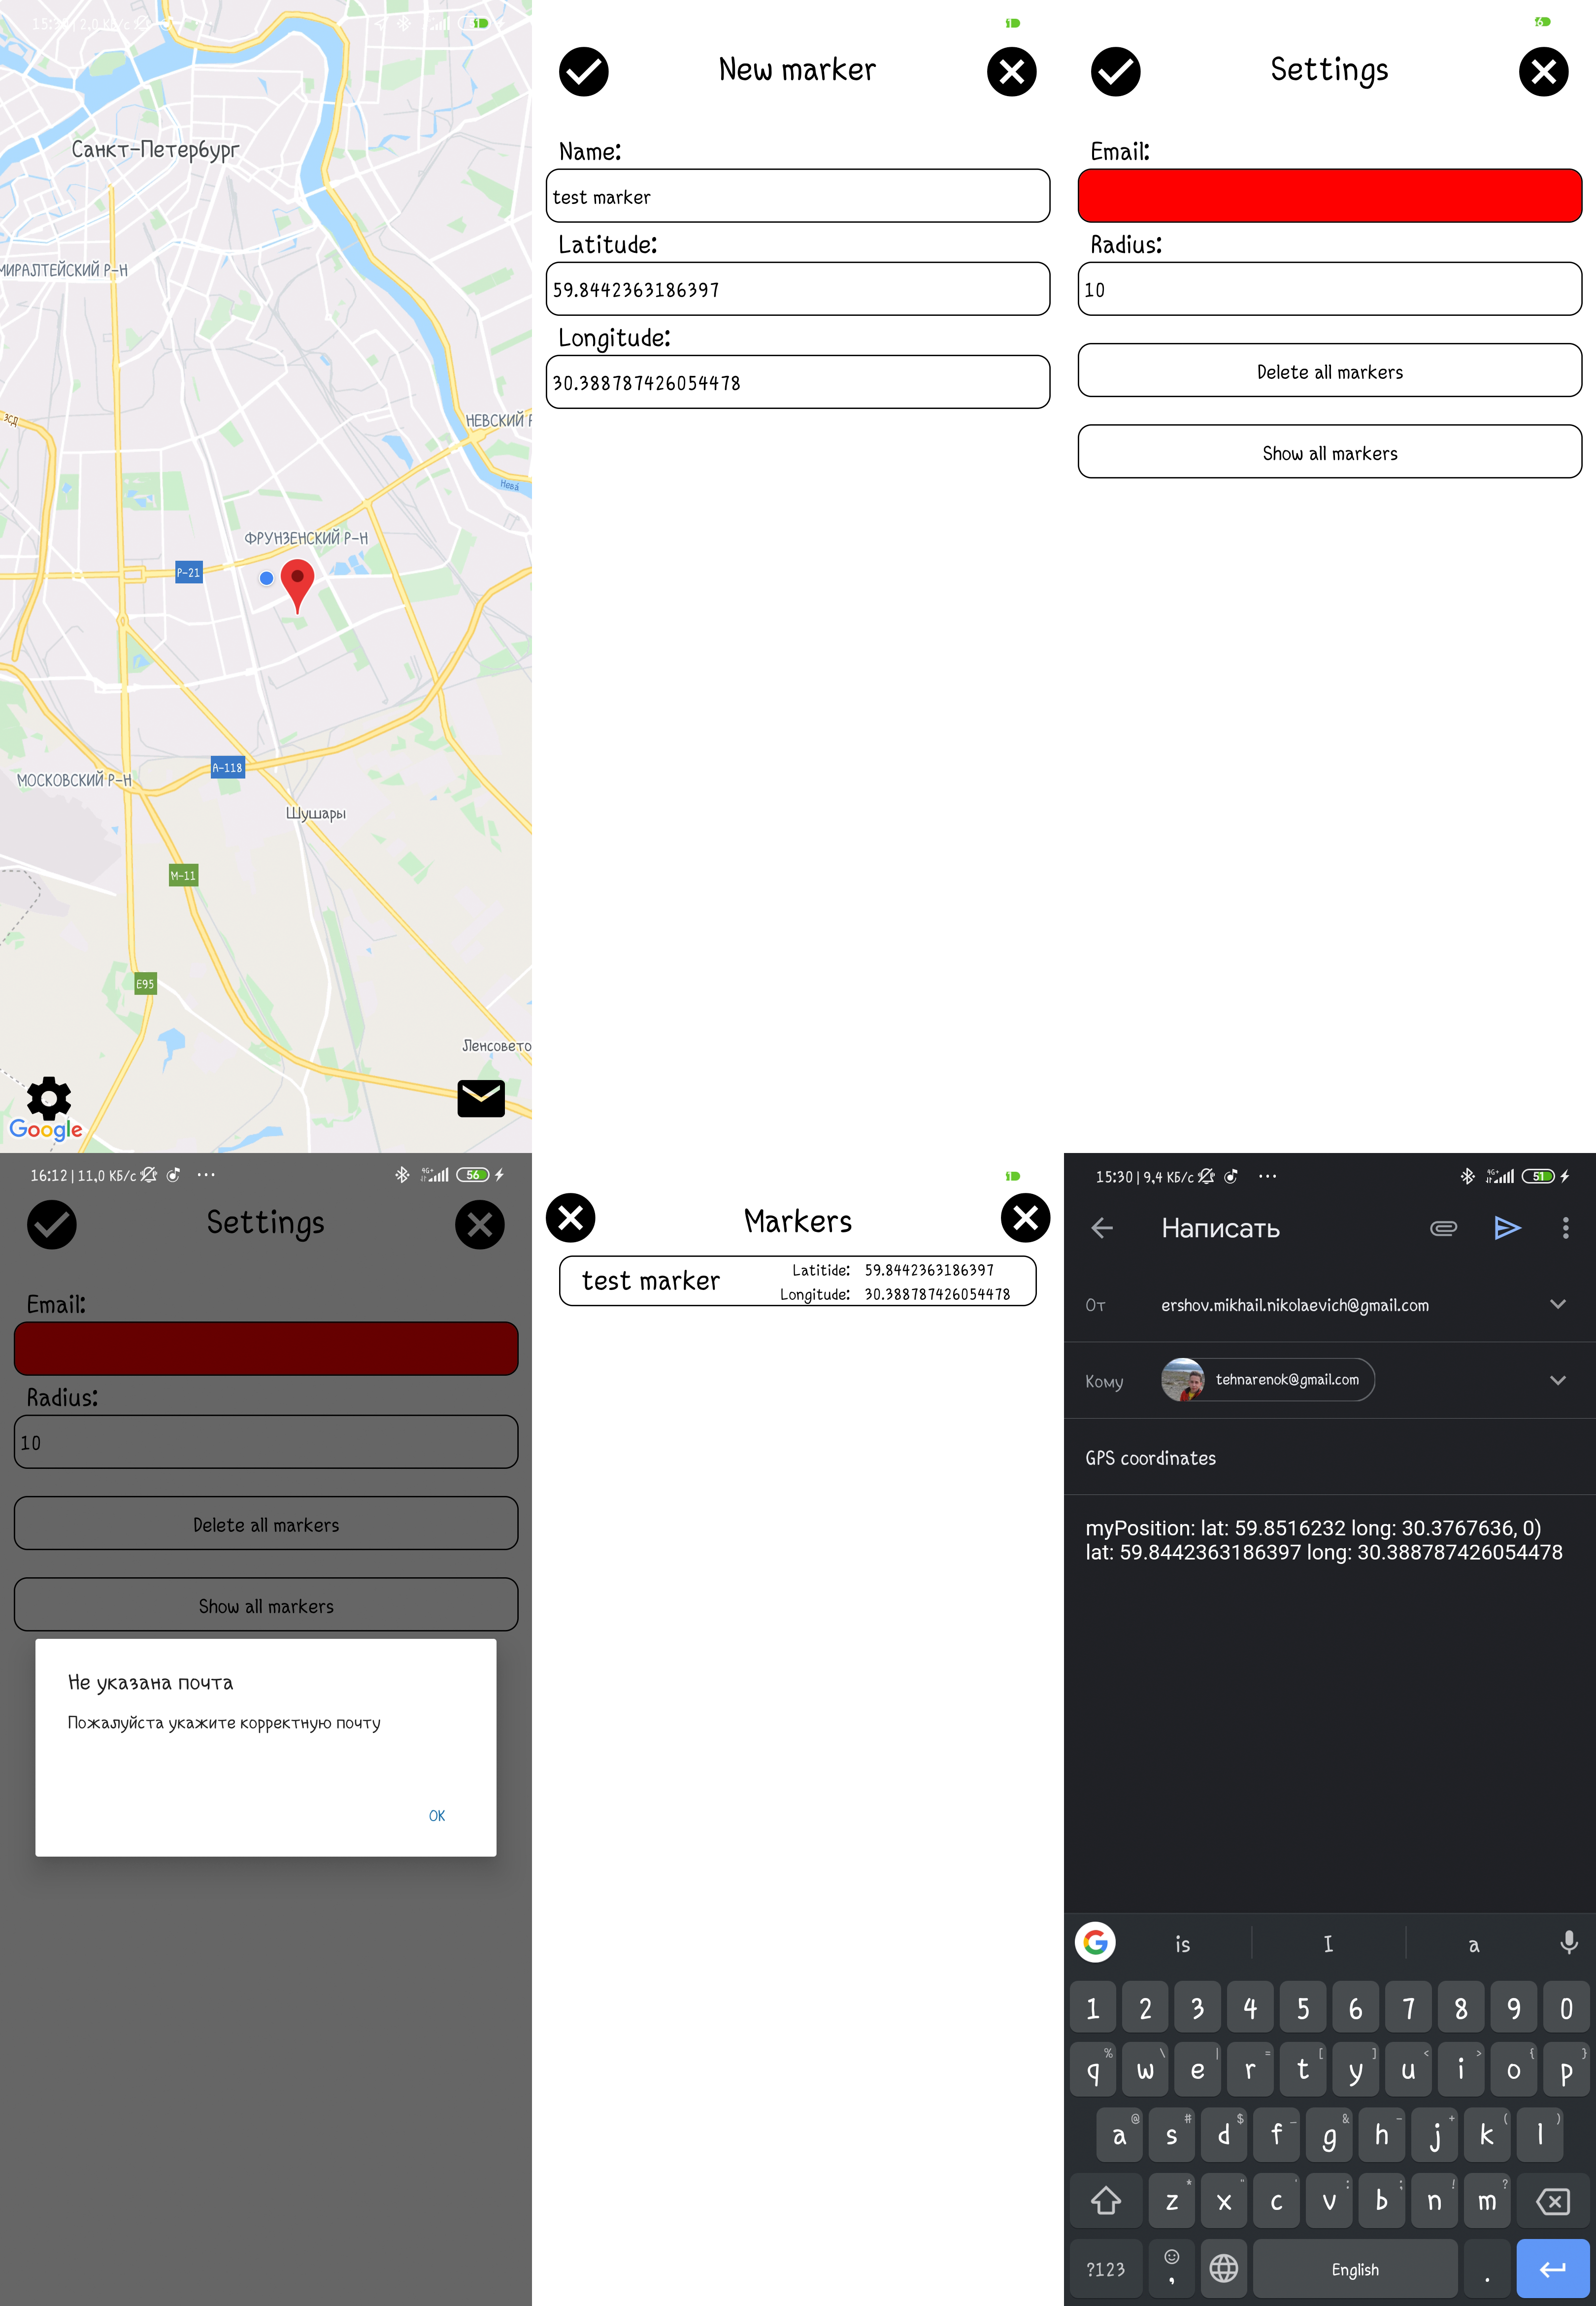
\includegraphics[width=\linewidth]{../screenshots/all.png}
\end{document}